% Figure from MATH 591 notes, section 17. Compile with the notes preamble.
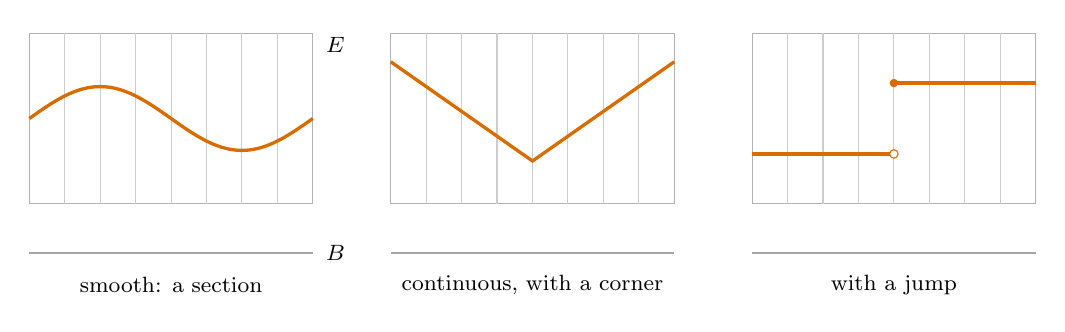
\begin{tikzpicture}[scale=0.9]
\foreach \k/\ttl in {0/{smooth: a section}, 1/{continuous, with a corner}, 2/{with a jump}} {
\begin{scope}[xshift={\k*5.1cm}]
\draw[gray!60] (0,0) rectangle (4,2.4);
\foreach \x in {0.5,1,1.5,2,2.5,3,3.5} \draw[gray!40] (\x,0) -- (\x,2.4);
\draw[thick, gray!70] (0,-0.7) -- (4,-0.7);
\node[font=\footnotesize] at (2,-1.15) {\ttl};
\end{scope}
}
\node[font=\footnotesize, anchor=south west] at (4.05,2.0) {$E$};
\node[font=\footnotesize, anchor=west] at (4.05,-0.7) {$B$};
\draw[orange!85!black, very thick, domain=0:4, samples=60, smooth] plot (\x,{1.2+0.45*sin(\x*90)});
\begin{scope}[xshift=5.1cm]
\draw[orange!85!black, very thick] (0,2.0) -- (2,0.6) -- (4,2.0);
\end{scope}
\begin{scope}[xshift=10.2cm]
\draw[orange!85!black, very thick] (0,0.7) -- (2,0.7);
\draw[orange!85!black, very thick] (2,1.7) -- (4,1.7);
\fill[orange!85!black] (2,1.7) circle (1.7pt);
\draw[orange!85!black, fill=white] (2,0.7) circle (1.7pt);
\end{scope}
\end{tikzpicture}
